% Preambule
\documentclass[11pt,a4paper,twoside,openright]{book}

% Standard packages
\usepackage{amsmath, amsthm, amssymb, graphicx}
\usepackage[utf8]{inputenc}

% PDF link
\usepackage[pagebackref]{hyperref}
\hypersetup{
   bookmarks=true,					% show bookmarks bar?
   unicode=false,					% non-Latin characters in Acrobat's bookmarks
   pdftoolbar=true,					% show Acrobat's toolbar?
   pdfmenubar=true,					% show Acrobat's menu?
   pdffitwindow=true,				% page fit to window when opened
   pdftitle={Thse de doctorat},		% title
   pdfauthor={Vincent Garcia},		% author
   pdfsubject={Thse de doctorat},	% subject of the document
   pdfnewwindow=false,				% links in new window
   pdfkeywords={},					% list of keywords
   colorlinks=true,					% false: boxed links; true: colored links
   linkcolor=red,					% color of internal links
   citecolor=green,					% color of links to bibliography
   filecolor=magenta,				% color of file links
   urlcolor=cyan					% color of external links
}

% Paths to figures
\graphicspath{{./figures/}}


% Style: By removing the following line, the style used is the basic book style
% Modification of marges
\addtolength{\oddsidemargin}{+1cm}
\addtolength{\evensidemargin}{-1cm}


% Use this package to modify part, chapter, and section style
\usepackage{titlesec}


% Modification of part style
\titleformat{\part}[display] 
{\Large \scshape} 
{	\filcenter
	\Huge
	\textbf{\partname}}
{30pt}
{	\titlerule[3pt]
	\vspace{30pt}
	\huge}
[]


% Modification of chapter style
\titleformat{\chapter}[display] 
{\bfseries \Large \scshape} 
{\center - \ \chaptertitlename \ \huge \thechapter \Large \ -} 
{1ex} 
{	\titlerule%
	\vspace{1pt}% 
	\titlerule%
	\vspace{2ex}% 
	\filcenter} 
[	\vspace{2ex} 
	\titlerule
	\vspace{2ex}
]


% Modification of section style
\titleformat{\section}
{\Large \scshape} 
{	\textbf{\S\ \thesection}}
{.5em}
{}
[	\vspace{1ex}] 


% Modification of header and footer style
\usepackage{fancyhdr}
\pagestyle{fancy}
\fancyhf{}
\fancyhead[RE]{\nouppercase\leftmark}
\fancyhead[LO]{\nouppercase\rightmark}
\fancyhead[LE,RO]{\thepage}
\renewcommand{\headrulewidth}{1pt}
\renewcommand{\footrulewidth}{0pt}


% Modification of caption style
\usepackage[labelfont=bf,textfont={it,rm}]{caption}


% Document
\begin{document}

    % Roman numbering
    \frontmatter 

    % Cover page
    \thispagestyle{empty}

\thispagestyle{empty}
\enlargethispage{3cm}
\vspace*{-2cm}
\hspace*{-2.9cm}
\begin{minipage}[t]{17cm}
	\centering

\LARGE{\textbf{University of FarFarAway}}\\
\vspace{1cm}

\textsc{Some text in small capitals}\\
\vspace*{0.3cm}
\large{\textit{Some other text in italic}}\\

\vspace*{0.9cm}
\huge{\textbf{THESIS}}\\

\vspace*{1.2cm}
\normalsize{Some text}\\
\vspace*{0.3cm}
\Large{\textbf{Some bold text}}\\
\vspace*{0.3cm}
\normalsize{Some text}\\
\vspace*{0.3cm}
\normalsize{Some text}\\

\vspace*{0.9cm}
\normalsize{presented by}\\
\vspace*{0.3cm}
\Large{Vincent \sc{Garcia}}\\

\vspace*{0.5cm}
\normalsize{Some text again}\\

\vspace*{1.5cm}
\rule{\textwidth}{3pt}\\
\vspace*{0.8cm}
{\LARGE\textsc{This is the title of this thesis}}\\
\vspace*{0.5cm}
\rule{\textwidth}{3pt}\\

\normalsize

\vspace*{1.5cm}
Some test again and again\\

\vspace*{0.7cm}
Last text before the jury

\vspace*{0.7cm}
\begin{tabular}{lll}
Bruce \textsc{Banner}    & Professor at Marvel University    \\
Peter \textsc{Parker}    & Professor at Marvel University    \\
Tony \textsc{Stark}      & Professor at Marvel University    \\
Matthew \textsc{Murdock} & Professor at Marvel University    \\
\end{tabular}

\end{minipage}

    % Table of content
    \setcounter{secnumdepth}{3}
    \setcounter{tocdepth}{3}
    \tableofcontents

    % Acknowledgments
    \include{acknowledgments}

    % Arabe numbering
    \mainmatter

    % Introduction
    \include{introduction}

    % Part 1
    \cleardoublepage
    \phantomsection
    \part{This is the first part of this thesis}
    \chapter{This is chapter one}


\section{This is section one}

This is some text. This is some text. This is some text. This is some text. This is some text. This is some text. This is some text. 
This is some text. This is some text. This is some text. This is some text. This is some text. This is some text. This is some text. 
The figure~\ref{fig:lena1} is the picture of Lena.
This is some text. This is some text. This is some text. This is some text. This is some text. This is some text. This is some text. 
This is some text. This is some text. This is some text. This is some text. This is some text. This is some text. This is some text. 
This is a reference to a paper~\cite{Garcia_2008_CVGPU}.

\begin{figure}[htbp]
    \centering
    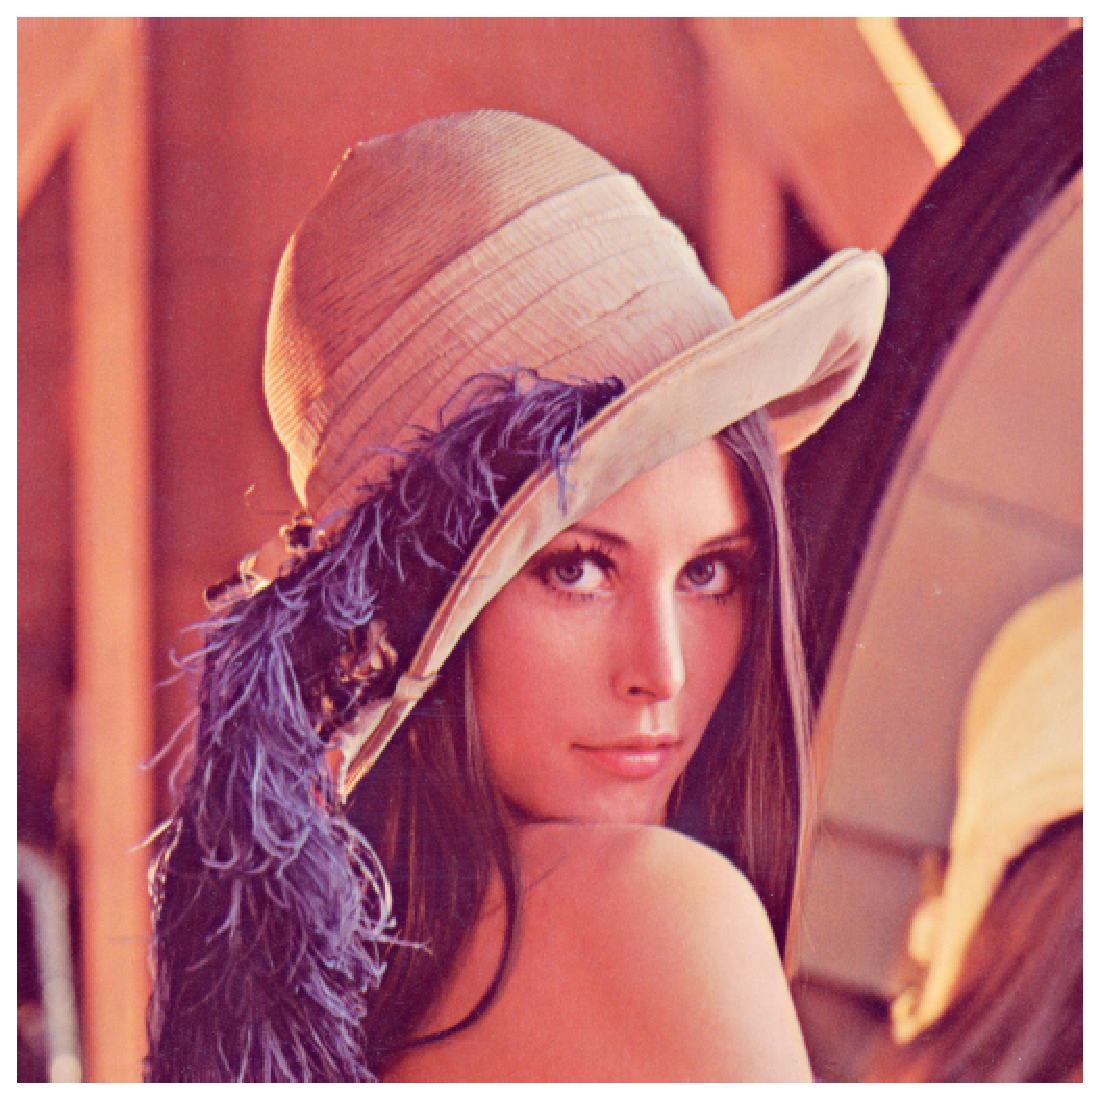
\includegraphics[width=0.4\linewidth]{lena}
    \caption{This is the caption of the figure Lena}
    \label{fig:lena1}
\end{figure}


\section{This is section two}

This is some text. This is some text. This is some text. This is some text. This is some text. This is some text. This is some text. 
This is some text. This is some text. This is some text. This is some text. This is some text. This is some text. This is some text. 
Equation~\ref{eq:normal1} is the formula of a multivariate normal distribution.
This is some text. This is some text. This is some text. This is some text. This is some text. This is some text. This is some text. 
This is some text. This is some text. This is some text. This is some text. This is some text. This is some text. This is some text. 

\begin{equation}
    f_X(x) = \frac{1}{ (2\pi)^{k/2}|\Sigma|^{1/2} } \exp\!\Big( {-\tfrac{1}{2}}(x-\mu)'\Sigma^{-1}(x-\mu) \Big)
    \label{eq:normal1}
\end{equation}


\section{This is section three}

This is some text. This is some text. This is some text. This is some text. This is some text. This is some text. This is some text. 
This is some text. This is some text. This is some text. This is some text. This is some text. This is some text. This is some text. 
The figure~\ref{fig:regularization1} shows some typical functions used in regularization.
This is some text. This is some text. This is some text. This is some text. This is some text. This is some text. This is some text. 
This is some text. This is some text. This is some text. This is some text. This is some text. This is some text. This is some text. 

\begin{figure}[htbp]
    \centering
    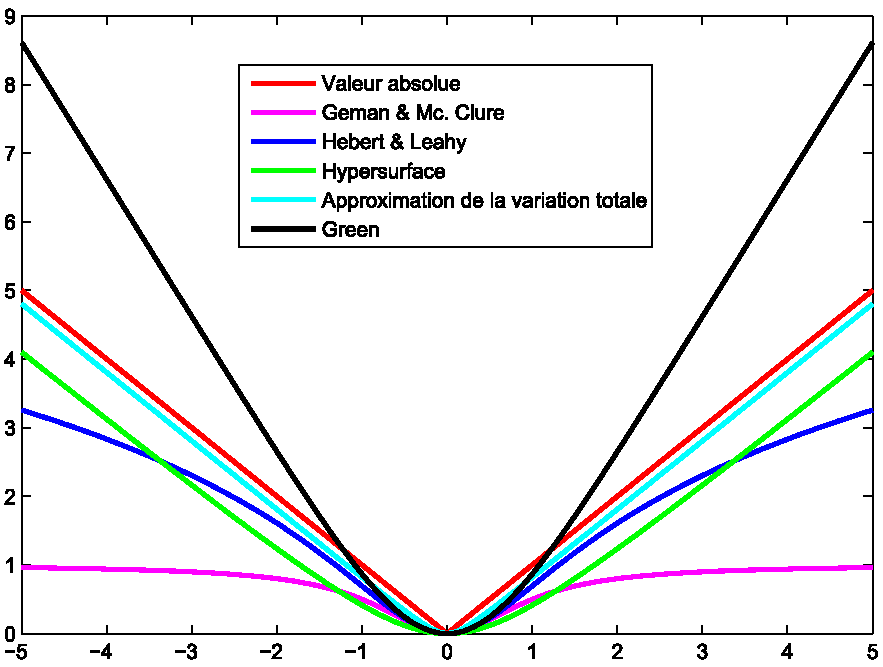
\includegraphics[width=0.7\linewidth]{regularization}
    \caption{Regularization functions}
    \label{fig:regularization1}
\end{figure}

    \include{chapter_02}

    % Part 2
    \cleardoublepage
    \phantomsection
    \part{This is the second part of this thesis}
    \include{chapter_03}
    \include{chapter_04}

    % Conclusion
    \cleardoublepage
    \phantomsection
    \part{Conclusion}
    \include{conclusion}

    % Annexes
    \appendix
    \cleardoublepage
    \phantomsection
    \part{Annexes}
    \include{annexe_01}
    \include{annexe_02}

    % Liste of figures
    \cleardoublepage 
    \phantomsection
    \addcontentsline{toc}{part}{List of figures}
    \listoffigures

    % Liste of tables
    \cleardoublepage 
    \phantomsection
    \addcontentsline{toc}{part}{List of tables}
    \listoftables

    % Bibliography
    \cleardoublepage 
    \phantomsection 
    \addcontentsline{toc}{part}{Bibliography}
    \bibliography{bibliography}
    \bibliographystyle{alpha}

\end{document}
